\documentclass[conference,a4paper]{IEEEtran}
\usepackage{cite}
\usepackage{amsmath,amssymb,amsfonts}
\usepackage{graphicx}
\usepackage{textcomp}
\usepackage{xcolor}
\usepackage[hidelinks]{hyperref}


\begin{document}

\title{Visual Dock-Velocity Feedforward for ROV Docking to a Moving Station: Failure Mechanism and Ego-Motion-Aware Estimation}

\author{\IEEEauthorblockN{1\textsuperscript{st} Chak Wang Choi}
\IEEEauthorblockA{\textit{School of Mechanical and Manufacturing Engineering} \\
\textit{UNSW Sydney}\\
Sydney, Australia \\
z5413670@ad.unsw.edu.au}
\and
\IEEEauthorblockN{2\textsuperscript{nd} William J.B. Midgley}
\IEEEauthorblockA{\textit{School of Mechanical and Manufacturing Engineering} \\
\textit{UNSW Sydney}\\
Sydney, Australia \\
w.midgley@unsw.edu.au\\
ORCID: 0000-0003-3786-1691}
}

\maketitle

\begin{abstract}
Moored and suspended docking stations inherit wave motion, so the terminal visual stage of underwater docking must track a moving target. Dock-velocity feedforward should help, but the velocity must be estimated from a camera on the moving vehicle. We report simulated docking of a BlueROV2 onto a station swaying with 0.1 m amplitude at periods from 20 to 6 s, with a passive-marker vision pipeline in the loop. A purely reactive baseline succeeds down to 8 s motion period, whereas a constant-velocity estimator with feedforward degrades at 10 s and fails at 8 and 6 s. In the failures, the estimated dock motion reaches 18 to 52 times the true amplitude, correlates with the vehicle's own position rather than with the dock, and is not eliminated by process-noise retuning. Camera measurements carry correlated error that the filter interprets as target velocity. Feeding this estimate into the control command introduces an unintended feedback coupling between vehicle motion and estimated dock motion. We propose an ego-motion-aware relative-position estimator, in which vehicle velocity enters the process model, and evaluate it against the reactive baseline, the original constant-velocity feedforward method, and an oracle feedforward case over a range of dock periods and navigation-error levels.
\end{abstract}

\begin{IEEEkeywords}
underwater docking, remotely operated vehicle, visual servoing, moving target, Kalman filter, velocity feedforward, ego-motion
\end{IEEEkeywords}

\section{Introduction}

Docking lets a resident underwater vehicle recharge and offload data without surfacing. The riskiest part of docking is in the final metres, where localisation is done using the forward camera. Real stations are rarely still: a suspended tether management system follows its vessel's heave \cite{trslic2020vision}, and a moored station follows the wave orbital motion at its depth. That motion decays with depth at a rate set by period, so a dock at continental-shelf depth still moves of order 0.1~m at the 5 to 20~s periods that carry wave energy \cite{holthuijsen2007waves}; the mean sea off New South Wales is 1.6~m at 8~s \cite{short1992wave}.

Docking control literature treats the dock as a fixed pose. Trslic et al.\ servoed reactively on the latest measured pose \cite{trslic2020vision} and later predicted cage heave, but from a pressure sensor on the cage and offline \cite{trslic2020neuro}. To our knowledge no prior work estimates a dock's wave-frequency motion onboard, through vision alone, from a vehicle that is itself moving, and closes the loop on that estimate. This paper does so for the passive-marker terminal stage of a low-cost ROV's docking manoeuvre, and reports that a constant-velocity (CV) dock estimator feeding forward a velocity, fails in an instructive way. We characterise the failure, propose a minimal estimator correction, and set out the comparison the full paper will report.

\section{System and Na\"{\i}ve Feedforward Architecture}

The vehicle is a BlueROV2 Heavy in Gazebo with the production ArduSub firmware software-in-the-loop \cite{blue2024software}. Nine size-graded ArUco markers \cite{garrido2014automatic} on the dock face allow pose estimation from 5~m. Detections are fused by inverse-variance weighting after spatial-consensus outlier rejection. The fused pose feeds a nine-state error-state Kalman filter over dock position, dock velocity and a small-angle attitude correction, run either \emph{static}, with zero velocity process noise (a constant-position filter), or \emph{sway}, with white-acceleration noise that estimates dock velocity. A supervisory state machine sequences coarse approach, fine align-then-advance and seat, with position-based visual servoing on the body-frame pose error. In the sway regime the filter velocity is rotated into the body frame, clamped, ramped in with distance and applied as feedforward through a command channel with about 240~ms of identified lag.

The dock velocity $\hat{v}_d$ is estimated through:
\begin{equation}
\text{camera} \rightarrow (\hat{p}_v,\hat{q}_v) \rightarrow \hat{p}_d^{\,meas} \rightarrow \text{CV KF} \rightarrow \hat{v}_d \rightarrow \text{FF},
\label{eq:chain}
\end{equation}
where the vehicle's own estimated pose $(\hat{p}_v,\hat{q}_v)$ is used to reconstruct the dock position $\hat{p}_d^{\,meas}$ in the world frame. Therefore a temporally correlated vehicle-state error enters the measurement, violating the white-noise assumption \cite{barshalom2001estimation}.

\section{Docking Envelope and Failure Evidence}

The sweep covers periods $\{20,16,12,10,8,6\}$~s at 0.1~m orbital amplitude, three start phases per cell, replicated on a second host (Fig.~\ref{fig:pdock} shows one 38-trial sweep). A trial is successful if the vehicle enters the 0.15 m docking aperture without first contacting the surrounding structure.

\begin{figure}[t]
\centerline{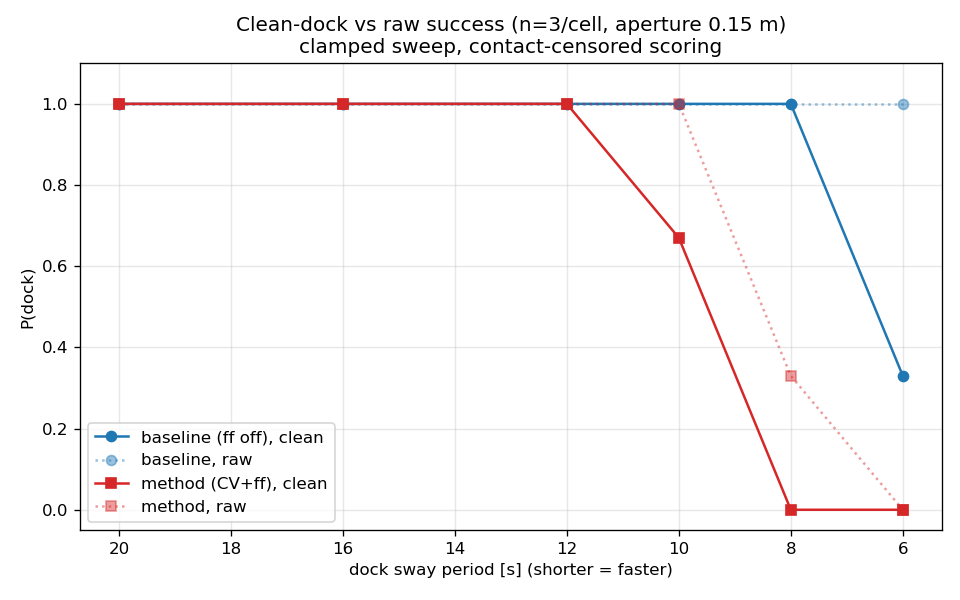
\includegraphics[width=0.70\columnwidth]{figures/clean_pdock.png}}
\caption{Docking success versus sway period, reactive baseline versus CV filter with feedforward; raw (dotted) and contact-censored (solid) scoring.}
\label{fig:pdock}
\end{figure}

In Fig.~\ref{fig:pdock} the baseline docks successfully in every trial down to 8~s; at 6~s two of three trials brush the aperture at 0.03 to 0.06~m/s. The CV-plus-feedforward method matches it down to 12~s, degrades at 10~s and fails at 8 and 6~s, the region of the mean New South Wales wave period.

The baseline has no velocity state and absorbs ego-motion leakage as position noise; its estimated sway amplitude is 0.7 to 0.9 times the truth in every run. The CV filter integrates the same leakage into a phantom dock velocity: the estimated amplitude is 2.4 to 5 times the truth in the runs that still dock and 18 to 52 times in the failures, where the estimate correlates 0.00 with the true dock and its excess motion 0.88 with the vehicle's own position. The feedforward injects this phantom velocity into the command. In the failed 8~s trial of Fig.~\ref{fig:failure}, loss of marker visibility causes the filter to propagate the incorrect dock-velocity estimate, and the estimated dock position diverges by about 1~m. The vehicle then tracks this erroneous estimate and fails to dock. The controller's internal alignment error remains between 0 and 0.017~m, while the ground-truth lateral error is 0.17 to 0.48~m.

\begin{figure}[t]
\centerline{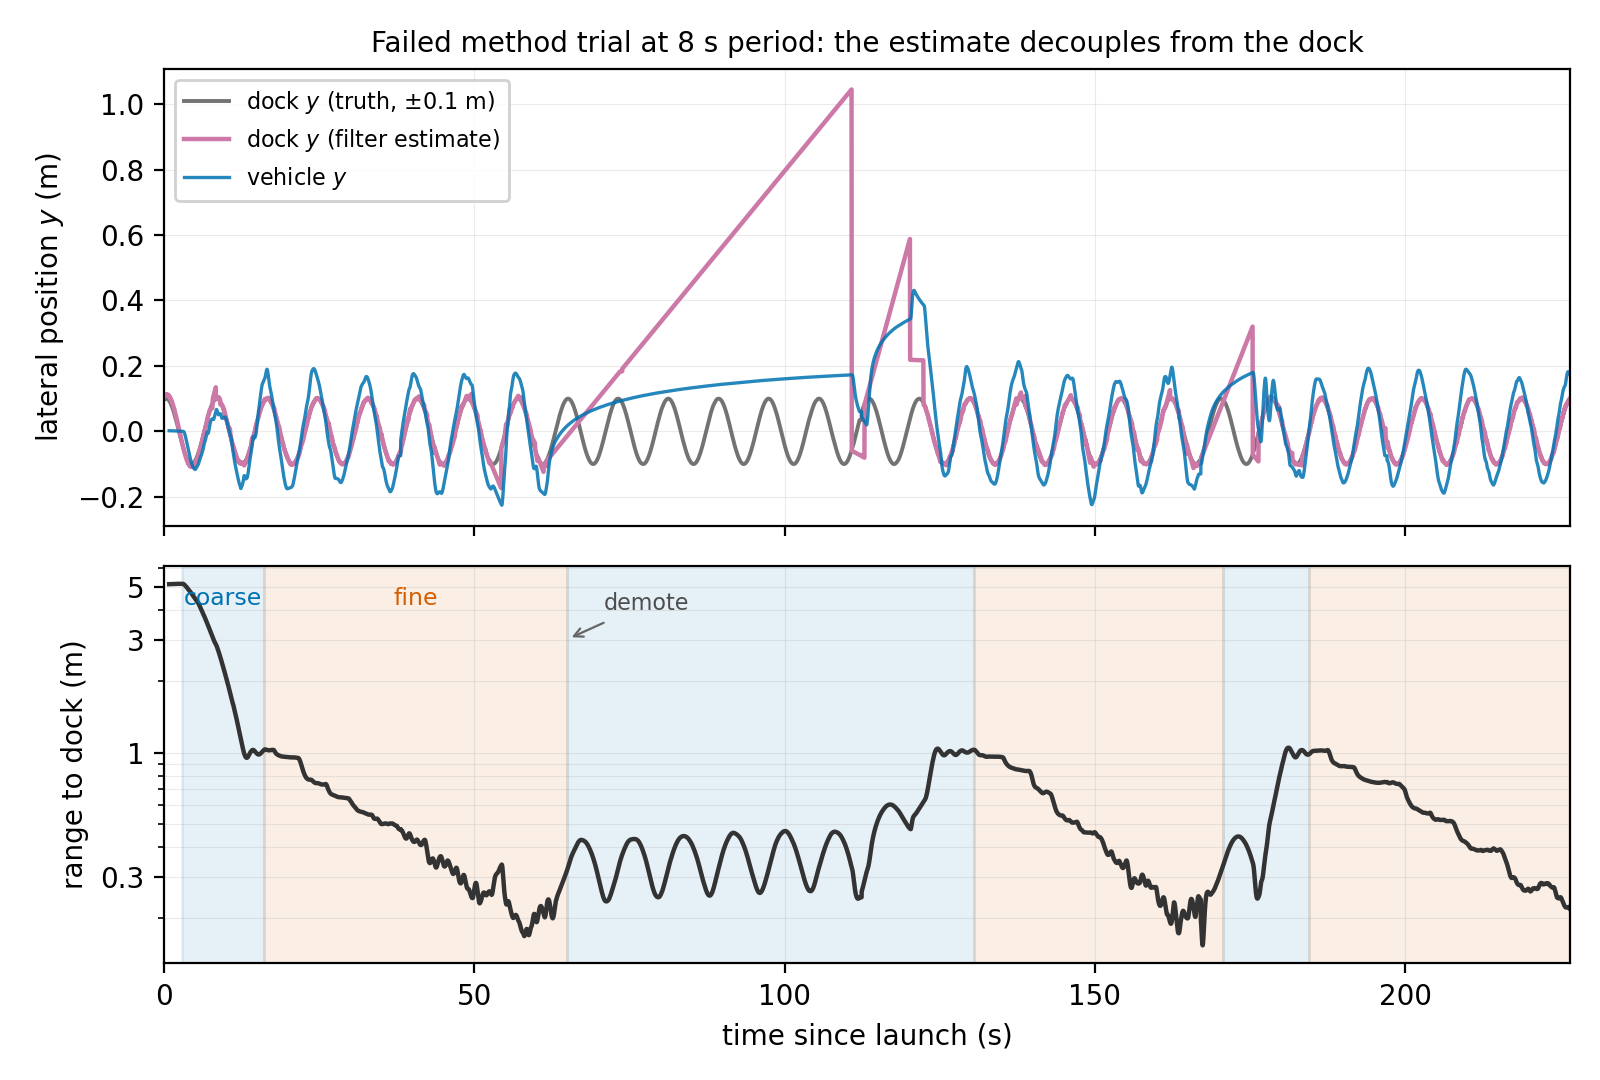
\includegraphics[width=0.70\columnwidth]{figures/rov_trajectory_failure.png}}
\caption{Failed CV-plus-feedforward trial at 8~s. Top: lateral position of true dock, dock estimate and vehicle. Bottom: range to dock, phases shaded.}
\label{fig:failure}
\end{figure}

Estimator tuning did not remove the failure. Velocity and covariance bounds limited the maximum estimation error, but the CV-plus-feedforward method still failed at shorter dock periods. Sweeping the acceleration-noise density from 0.02 to 0.16~m/s\textsuperscript{2} produced estimated dock-motion amplitudes 5 to 37 times the true value. The reactive baseline does not exhibit this behaviour because it does not estimate dock velocity. In the CV case, $\hat{v}_d = v_d + H_e(s)v_v + \eta$, where $H_e(s)$ represents coupling from vehicle motion into the dock-velocity estimate; feeding $\hat{v}d$ into the command therefore introduces an unintended feedback path with $L(s)=K{ff}G_p(s)H_e(s)$. The identified 240~ms command-to-velocity lag is consistent with the reduced performance at 8--10~s periods.


\section{Proposed Estimator and Evaluation Plan}

The proposed correction changes only the estimator's origin. The translational state becomes $x = [r,\;v_d]^T$ with $r = p_d - p_v$ the dock position relative to the vehicle in world-aligned axes,
\begin{equation}
r_{k+1} = r_k + (v_{d,k} - \hat{v}_{v,k})\,\Delta t + w_r, \qquad v_{d,k+1} = v_{d,k} + w_v,
\label{eq:rel}
\end{equation}
so vehicle velocity $\hat{v}_v$ enters as a known process input, and the measurement $z_k = r_k + \nu_k$ is the camera-relative translation rotated by attitude only; the vehicle world position is never added. Fusion, gating, bounds, controller, state machine and feedforward law are unchanged. In loop terms the corrected estimator should reduce $H_e$; oracle feedforward has $H_e = 0$.

The full paper will compare, under identical imperfect navigation, (A) the reactive baseline, (B) na\"{\i}ve CV plus feedforward, (C) the corrected estimator plus feedforward and (D) oracle feedforward from ground-truth dock velocity as a diagnostic bound, over the same periods with 8 to 12 phases at 6 to 12~s, and (A--C) three levels of correlated navigation error modelled as a first-order Gauss--Markov velocity bias. Oracle D separates estimator-limited from plant-limited failure: if D fails at short periods the plant is the limit; if D succeeds where B fails, estimation is; if C approaches D, the mechanism and fix are confirmed. Metrics are docking success rate, capture error and closing speed, and dock-velocity estimation error.

\section{Conclusion}

Dock-velocity feedforward for a moving station cannot be added to a static-dock pipeline as an afterthought: the estimator, the feedforward gain and the plant response form a loop that must be designed jointly, and a reactive baseline provides a robust fallback in the tested envelope. Because the failure is invisible to the system's own health signals, any deployment needs independent verification.

\bibliographystyle{IEEEtran}
\bibliography{refs}

\end{document}